\section{GitLab}
    GitLab je především systém pro správu repozitářů a vzniknul jako otevřená alternativa služby GitHub. Nabízí ale velmi kvalitní vlastní \CI a má nástroje podporující \CD. GitLab je poskytován jako \glstext{SaaS} a to jak v managed variantě, tak v placené self-hosted variantě. Existuje i fukčně velmi ořezaná self-hosted verze zdarma. Veřejné jádro je poskytované jako \textit{GitLab Community Edition}, placené části jsou vedeny jako \textit{GitLab Enterprise Edition}.

    Oficiálně GitLab podporuje celou řadu instalačních možností od balíčků pro klasické Linux distribuce, přes Docker kontejnery až po složitější šablony pro Kubernetes nebo OpenShift. Do podzimu 2018 byl GitLab distribuován jako monolitická aplikace, které se velmi obtížně škálovala a spouštěla distribuovaně v několika replikách. Podařilo se ale GitLab rozdělit na jednotlivé komponenty (gitaly: git repozitáře, gitlab-shell: HA api nad gitaly, mailroom: správa příchozích emailů, sidekiq, task-runner, unicorn: ruby webserver). Dále ma GitLab řadu externích závislostí: relační databázi (konkrétně PostgreSQL, podpora pro MySQL už neexistuje), key-value storage (Redis), úložitě pro objekty (AWS S3 nebo otevřená alternativa s kompatibilním api Minio). V oficiálním docker image, kterému říkají \textit{omnibus}, jsou všechny tyto závislosti přibalené. Nově vznikly separátní docker image pro každou GitLab službu zvlášť a šablony pro Kubernetes Helm, usnadnující jejich spuštění a konfiguraci.

    Protože jsou oba přístupy diametrálně odlišné, rozhodl jsem se nasadit GitLab jak v původním \textit{omnibus} variantě distribuované jako balíček pro Debian, tak ve variantě mikroslužeb v prostředí kontejnerů a porovnat obě varianty.

    \subsection{GitLab Omnibus}
        Instalace podle oficiální dokumentace je velmi jednoduchá. Jde jenom o přidání vlastního repozitáře a instalace balíčku \cite{gitlab-install-ubuntu}. Po instalaci je rovnou spuštěna celá aplikace a při přístupu na HTTP endpoint se rovnou zobrazuje dialog pro nastavení administrátorského hesla.

        Aplikaci lze konfigurovat na několika místech: z webového rozhraní, \code{gitlab.yml} a \code{gitlab.rb}). V každé části je bohužel trochu něco jiného. V rámci této práce jsem upravil konfiguraci v \code{gitlab.rb}, kde jsem nastavil externí \glstext{URL}, na kterou GitLab generuje externí linky (například v emailové komunikaci), počáteční heslo pro administrátora a především token, kterým se bude autentifikovat GitLab Runner obstarávající \CI.

    \subsection{GitLab mikroslužby}
        GitLab začal oficiálně na konci roku 2018 podporovat také nasazení do Kubernetes přes Helm \cite{gitlab-helm-chart}. Kubernetes je distribuovaný orchestrátor kontejnerů a Helm je balíčkovací aplikace. Každá komponenta GitLabu byla oddělena do samostatného docker obrazu a v Helm balíčku (\textit{Helm chart}) je pomocí Kubernetes zdrojů popsáno jak se dané kontejnery mají spouštět a jak jsou provázané. Teoreticky je možné kontejnery spouštět i ručně v jiném systému než Kubernetes, ale není to oficiálně podporované a neexistuje k tomu dokumentace.

        \todo{diagram}
        \missingfigure[figwidth=\columnwidth,figheight=7cm]{Architektura GitLab \label{pic:gitlab-architecture}}

        Hlavní výhody nasazení GitLabu přes mikroslužby jsou:
        \begin{itemize}
            \item Přehlednost. Administrátor přesně ví, jaké komponenty systém obsahuje. Jednotlivé části nejsou skryté v Omnibus balíčku, kde se těžko dohledávají logy.
            \item Metriky mohou přímo využívat exportery nasazené v clusteru. V Omnibus jsou k dispozici pouze metriky pro celý balík, nebo je musí další proces uvnitř exportovat. To je další komplexita a nekonzistence se zbytkem prostředí.
            \item Lepší škálovatelnost. Můžeme škálovat pouze některé komponenty. Navíc díky přesným metrikám můžeme škálovat vytížené komponenty dynamicky.
            \item Využití upstream služeb. Řada komponent, které GitLab využívá, jsou nezměněné aplikace třetích stran. To je například ElasticSearch, Redis a relační databáze. V Omnibus balíčku jsou přibalené; nelze je aktualizovat a pokud na to GitLab nemyslel, nelze je vyčlenit a použít externí službu. U mikroslužeb má administrátor plnou kontrolu nad tím, které služby nasadí a pro které například použije cloudovou managed variantu.
        \end{itemize}

        Instalace GitLabu jako mikroslužeb je oproti verzi Omnibus velmi komplikovaná. Vyžaduje minimálně uživatelskou znalost Kubernetes a velmi podrobnou znalost Helm. Dokumentace je zatím (k lednu 2019) nekompletní a hodně nastavení a jejich význam je nutné dohledávat v šablonách Helm chartu. Některé konfigurace nejsou podporovánu vůbec. Narazil jsem například na nutnost nakonfigurovat Redis clusteru s heslem \cite{gitlab-helm-issue-redis}. Například managed varianta od \glstext{AWS} podporuje přihlášení heslem pouze při použití \glstext{TLS} tunelu, protože bez něj se posílá heslo v plaintextu a nedává moc smysl vůbec heslo použít. To souvisí s tím, že GitLab mikroslužby jsou velmi nové; dá se očekávat, že čím víc firem bude takto GitLab nasazovat, tím lepší dokumentace a podpora pro různá prostředí vznikne.

    \subsection{GitLab \CI}
        \CI není přímo komponenta distribuovaná s GitLab, je ale dobře zaintegrovaná. Díky skvělému návrhu GitLab pouze vystavuje události na \glstext{API}. K API se může registrovat libovolné množství runnerů, které se periodicky \glstext{API} dotazují na nové práce ke spuštění \cite{gitlab-runner-registration}. Runner může běžet na stejném serveru jako GitLab, ale velkou výhodou je možnost spustit runner i na jiném vzdáleném serveru -- například pro mobilní aplikace se často používá Mac mini s macOS, které je pro kompilaci nezbytné. Při registraci runneru je možné ho přidělit pouze některým projektům podle tagu, nebo ho zveřejnit pro všechny projekty.

        Runner při získání práce z \glstext{API} má k dispozici soubor s definicí (obsah souboru \code{.gitlab-ci.yml} \cite{gitlab-runner-yaml}) a přístupové údaje k repozitáři. Architektura GitLab \CI se skládá z tzv. \textit{stages} (etapy) a \textit{jobs} (kusy práce) (obrázek \ref{pic:gitlab-ci-architecture}). Jeden push do repozitáře typicky vygeneruje jednu \textit{pipeline}, což je sada \textit{stages} a \textit{jobs} popsaná konfigurací \CI v daném commitu.

        \todo{diagram}
        \missingfigure[figwidth=\columnwidth,figheight=7cm]{Architektura GitLab \CI \label{pic:gitlab-ci-architecture}}

        \todo{rozepsat moznosti konfigurace: že to umi cache, dependencies z predchozich jobu, ze to jde vsechno pouze seriove a dependencies se nepouzivaji pro paralelizaci}\blind[1]

        V oficiální implementaci nabízí runner celou řadu možností, jak jednotlivé \textit{jobs} spouštět, tzv. \textit{executors} \cite{gitlab-runner-config}. Základní je \code{shell}, při kterém neexistuje prakticky žádná izolace procesů a čištění prostředí. Jakékoliv závislosti, které je potřeba instalovat do sytému, ovlivňují všechny ostatní procesy na stejném serveru. Procesy běží pod neprivilegovaným uživatelem \code{gitlab-runner}, takže je lepší potřebné závislosti nainstalovat předem administrátorem. Tento executor může bbýt vhodný pro dedikované prostředí pokud zajistíme, že tento server využívá pouze jeden projekt, případně pouze důvěryhodné nekolidující projekty. Velmi podobně funguje executor \code{ssh}, který místo na lokálním stroji spouští příkazy vzdáleně. Na cílovém stroji nejsou potřeba žádné závislosti (samozřejmě s výjimkou ssh serveru); v cloudovém prostředí může být praktické mít čisté virtuální stroje, na které se pak ssh runner připojuje. Dále lze ssh executor využít pro systémy, na kterých runner nemůže běžet lokálně. Velkou nevýhodou tohoto prostředí je nízká opakovatelnost. Jelikož se všechny joby mohou navzájem ovlivňovat a hostující systém se průběžně mění, starší joby které dřív končili úspěšně už nemusí fungovat. Ostatní executory tento problém do značné míry eliminují.

        Zbylé executory mají kompletní izolaci všech jobů. Možnosti \code{parallels} a \code{virtualbox} startují pro každý job nový virtuální stroj, z jednoho obrazu podle konfigurace runneru. Kontejnerizace jobů je nabízena v executoru \code{docker}: pro každý job je možné zvolit vlastní image. Varianta \code{kubernetes} je pro runner běžící v Kubernetes clusteru a vytváří pro každý job nový pod. Všechny tyto executory mají dobře opakovatelné joby. Pokud nezměníme obraz virtuálního stroje, případně pokud používáme stále stejný docker image, budou až na případné externí závislosti joby spuštěné identicky jako dřív.

        \label{sec:gitlab-ci-docker}
        Nastavení \CI se dále komplikuje při buildu Docker obrazů. Při použití většiny executorů máme dvě možnosti. První varianta je použít hostitelský Docker. U \code{shell} (a potažmo \code{ssh}) executoru stačí vyřešit oprávnění (typicky je potřeba přidat uživatele \code{gitlab-runner} do skupiny \code{docker}). U \code{docker} případně \code{kubernetes} executoru můžeme mountnout ovládací Unix socket \code{/var/run/docker.sock} do našeho kontejneru. Pro virtuální stroje by teoreticky šel socket mountnout také, ale když přijdeme o izolaci nemusíme pak \glstext{VM} používat vůbec. Nevýhodou tohoto řešení je, že všechny aplikace využívající \CI vidí obrazy a cache ostatních aplikací. Pokud se jedna z aplikací přihlásí do vzdáleného registru a stáhne nějaký soukromý obraz (\code{docker pull}), všechny ostatní aplikace tento obraz pak vidí a mohou ho číst i přesto, že nemají k vzdálenému registru oprávnění. Podobně jako při použití \code{shell} executoru tak musíme při sdílení Docker daemonu na \CI stavět pouze důvěryhodné aplikace.

        Druhou variantou buildu Docker obrazů je tzv. \textit{Docker in Docker} (\glstext{DinD}). To je Docker démon zabalený do Docker kontejneru. Při spuštění stále sdílí Linuxové jádro s hostitelským systémem, ale samotný Docker proces je izolovaný: má samostatný seznam procesů, vlastní limity a oddělenou build cache. \glstext{DinD} může být spuštěný právě pro jeden job. Ukázková specifikace pipeline pro Docker v kontejnerovém prostředí je popsána \pfxref{v kódu}{fig:gitlab-dind}.

        \begin{figure}[hb]
            \begin{minted}[frame=lines,framesep=2mm,linenos]{ruby}
services:
  - "docker:dind"

variables:
  DOCKER_HOST: "tcp://docker:2375"

build:
  stage: build
  script:
    - docker build --tag demo-build .
            \end{minted}
            \caption{Ukázkový soubor \code{.gitlab-ci.yml} pro nastavení \glstext{DinD}.}
            \label{fig:gitlab-dind}
        \end{figure}

        Při samostatně spuštěném \glstext{DinD} pro každý build máme perfektní izolaci všech klientů, ale přicházíme o některé výhody Dockeru, konkrétně o stažené obrazy a cache předchozích buildů. To je známý problém a GitLab ho bez úspěchu řeší už několik let \cite{gitlab-docker-artifact-caching}. Největší výhoda tohoto řešení je perfektní dostupnost: každá pipeline má vlastní Docker a případné aktualizace se dějí na úrovni změny obrazu v \code{.gitlab-ci.yml}. Přes GitLab mechanizmus pro cachování lze uložit Docker data a při dalším jobu je opět nahrát do nového Docker daemona \cite{patel-docker-cache}. Toto řešení je ale velmi pomalé. Obrazy včetně cache budou běžně kolem stovek megabajtů a zapisujeme je dokonce hned čtyřikrát: jednou na disk při exportu, potom do GitLab cache což je často externí objektové úložiště (jako je AWS S3) a po čtvrté při načítání do prázdného Dockeru. Pro aplikace s extrémně dlouhým buildem v řádu desítek minut to může být přínosné, ale pro typické webové aplikace na které se tato práce soustředí není toto řešení vhodné.

        Velmi úspěšně lze ale \glstext{DinD} provozovat jako dlouhožijící službu oddělenou od samotné \CI pipeline. Získáme tím tak výhody obou řešení a veskrze eliminujeme všechny nevýhody. Pro každou skupinu navzájem si věřících aplikací spustíme samostatný \glstext{DinD} proces. Ten může běžet na hostitelském serveru s \CI nebo libovolném externím. V daných pipeline specifikacích pak stačí neuvést \code{services: "docker:dind"} a nakonfigurovat proměnnou \code{DOCKER\_HOST} (například \code{tcp://group-7.external-docker.local:2375}). Každá skupina aplikací uvidí pouze svoje obrazy a bude mít persistentní cache. Nevýhodou tohoto řešení je vysoká komplexita. Je nutné nějakým způsobem zajistit, aby se k Docker socketu mohly připojit pouze autorizované aplikace. Na to je praktické použít nějakou pokročilou abstrakci, například Network Policies v Kubernetes. Samotná \glstext{ACL} logika může být v síťové vrstvě jako je například Weave, Contrail nebo Calico, nebo v samostatném dedikovaném firewallu.

    \subsection{Podpora \CD praktik}
        Ve svém marketingovém copy se GitLab prezentuje jako jednotný systém pro \CICD, monitoring a bezpečnost. Jak jsem popsal v předchozí sekci, \CI nabízí GitLab perfektní. Co se týče podpory \CD, funkce GitLabu jsou omezené:

        \textbf{Environments} přináší přehled všech prostředí (například beta, produkce, \ldots) a nasazení do těch to prostředí \cite{gitlab-environments}. Užitečná je možnost spouštět z tohoto zobrazení deploy znovu. Lze spustit i deploy nějaké starší verzi a udělat tak rollback. Při vhodném rozdělení pipeline na build a deploy je spuštění z tohoto přehledu je rychlejší, než spouštět celou pipeline. GitLab nenabízí žádnou možnost jak rollback omezit a je pouze na uživatelých, aby nespustili rollback na nějakou starou nekompatibilní verzi.
        \textbf{Review Apps} jsou prodávány jako systém, díky kterému lze nasadit zkušební verze aplikace do oddělených dynamických prostředí \cite{gitlab-review-apps}. Prakticky to jde udělat v libovolném \CI systému; pro vybrané větve se spustí deploy a dynamicky se předá nějaký identifikátor pro veřejnou \glstext{URL} a další konfiguraci, to může být například název dané větve. Jediné co přináší GitLab je podpora pro dynamické \textit{Environments} bez nutnosti programovat to přes \glstext{API}, a tlačítko \textit{Stop} v webovém rozhraní, které spustí pipeline job která má na starost job vypnout. Veškerá praktická implementace je ale na vývojáři: GitLab neřeší nasazení a vypnutí aplikace, pouze zavolá uživatelem definovaný job.
        \textbf{Auto DevOps} \cite{gitlab-auto-devops}. Tato kontroverzní \cite{gitlab-auto-devops-forum} funkce GitLabu je zjednodušeně řečeno jenom hodně komplikovaný \code{.gitlab-ci.yml} soubor, který uživatel nevidí a použije se, pokud není v repozitáři jiná konfigurace pipeline. Auto DevOps pipeline má kolem 1000 řádek a obsahuje pokročilé Yaml konstrukce jako jsou reference a vnořování, které zhoršují čitelnost. Navíc do toho míchají bash scripty a využívají docker kontejnerů. Celá pipeline je ve výsledku hodně složitá. Auto DevOps podporuje pouze nasazování do Kubernetes clusteru. Build aplikace funguje jenom když je aplikace samotná stavěná pomocí \code{Dockerfile}. Distribuce obrazu musí být pomocí GitLab Container Registry. Deploy probíhá pomocí Helm. Lze použít výchozí Helm Chart distribuovaný s Auto DevOps, nebo použít vlastní. Ve vlastním Helm Chartu, resp. v konkrétních Kubernetes zdrojích, lze pak ručně nakonfigurovat vlastnosti rolling-update konkrétní aplikace a obecně škálování a dostupnost. Ve výchozím nastavení není explicitně rolling-update nakonfigurován.

        Ze všech systémů které řeší \CI a zároveň \CD je GitLab se svým Auto DevOps nejdál. Je ale velmi dogmatický a nebude fungovat s žádnou odchylkou v infrastruktuře.

        Drobnější funkce GitLabu podporující \CD:
        \begin{itemize}
            \item Možnost spouštět vybrané joby v pipeline pouze manuálně. Jedno z možných použití je deploy aplikace z \code{master} větve, kde vývojář může ručně spustit job pro deploy po doběhnutí předchozích automatických jobů. Bohužel všechny automatické joby definované v následujících stages se spouští bez čekání na manuální job a to i tehdy, když mají definované závislosti na manuálním jobu \cite{gitlab-issue-manual-job}.
            \item Plánované spuštění pipeline. Přestože lze build spouštět programaticky z \glstext{API} z libovolného cronu, je užitečné že to má GitLab přímo implementované. Typické použití je tzv.~\textit{nightly build}.
            \item \textbf{Web terminals} umožňují připojit se do aplikačního kontejneru v Kubernetes clusteru. Podobně jako u Auto DevOps je tato integrace dogmatická a nekompatibilní s klasickým použitím Kubernetes labels \cite{gitlab-issue-k8s-deploy}.
        \end{itemize}

    \subsection{Open-source}
        GitLab je vyvíjen jako otevřený software, v tom smyslu, že veškerý kód je veřejně čitelný. Některé části jsou opravdu open-source i co se licence týče: GitLab \glstext{CE} je pod \glstext{MIT} licencí. Jiné části, například GitLab \glstext{EE}, jsou pod vlastní licencí. Licence dokonce ani nedovoluje \glstext{EE} verzi provozovat bez zakoupené licence.

        Příspěvky a návrhy na změny kódu od lidí mimo GitLab Inc. jsou možne, ale vesměs ignorované. Jako přispěvatel jsem hodně cítil, že firma GitLab je čistě remote a nemá žádné kanceláře a tým na jednom místě \cite{gitlab-team}. Většina návrhů na změnu -- od jednořádkových oprav po drobnější funkční úpravy -- co jsem poslal zůstala bez povšimnutí. To je tím spíš mrzuté, když razí cestu „minimum konfigurace, radši pošlete návrh na úpravu kódu pro všechny“ \cite{gitlab-no-custom}.

        U jednoho úkolu do kterého jsem se víc zapojil trvalo rok a půl začlenit drobnou změnu. Na tyto změny čekalo několik desítek firem. Šest vývojářů poslalo nezávisle na sobě návrhy na změnu. Změny byly vesměs triviální, bez dopadu na ostatní části kódu, byly otestované a dobře zdokumentované. Po opakovaném urgováním přes oficiální kanál podpory se u úkolu vyjádřil zaměstnanec GitLab. Bohužel se pouze zeptal, kdo má tuto část kódu na starost a tím na dva měsíce úkol opět usnul. Když se po dalším urgování přes podporu úkolu někdo chopil, zadání vesměs nepochopil a snažil se protlačit nepoužitelné řešení. Nechal si naštěstí problém znovu vysvětlit a řešení přehodnotil. Nakonec byl celý problém vyřešen a změny jsou zařazeny do vydání 11.8, tedy skoro 2 roky po otevření úkolu. Celé vlákno je veřejně na GitLab Issue Trackeru \cite{gitlab-issue-slow}. Podobnou zkušenost mám i z několika dalších GitLab projektů, včetně aktivně vyvíjeného GitLab Helm Chart.

    \subsection{Rozšiřitelnost}
        \todo{Má gitlab nějaké pluginy, dá se pro to scriptovat, jak je to bezpečné a jednoduché?}\blind[1]

    \subsection{Zálohování}
        \todo{Zálohování a restore}\blind[1]

    \subsection{Zabezpečení}
        Podle \glstext{CVE} Details měl GitLab nejvíc kritické problémy -- hodnocené podle podle \glstext{CVSS} -- zjištěné v posledním roce (2018) \cite{cve-gitlab}. To může souviset s exponenciálním růstem, který zažili díky \code{\#movingtogitlab} a akvicizi firmou Microsoft \cite{gitlab-growth}. Není zatím jasné, jestli dramatický nárůst počtu uživatelů přilákal bezpečnostní analytiky, nebo jestli bezpečnostní problémy jsou výsledkem zrychleného vývoje a zhoršení kvality produktu.

        \todo{Jak dlouho trvá gitlabu opravit cve a zverejnit fix?}

        Správa problémů (\textit{issues}) u projektů na GitLabu má možnost vytvořit nový záznam v důvěrném režimu. Takové problémy jsou pak viditelné pouze pro správce repozitáře. To je vhodné pro \textit{responsible disclosure} (zodpovědné zveřejnění) bezpečnostních chyb. GitLab toto úspěšně používá i pro vlastní projekty.

        GitLab zavádí v kontextu \CICD nový pojem \textit{continuous security testing} (kontinuální bezpečnostní testování) \cite{gitlab-app-security}. Na rozdíl od testování po začlenění změn a nasazení, GitLab umožňuje každému vývojáři deploynout danou větev verzovacího systému do vlastního testovacího prostředí. To je znázorněno \pfxref{v diagramu}{fig:gitlab-review-cycle}.

        \begin{figure}[hb]
            \centering
            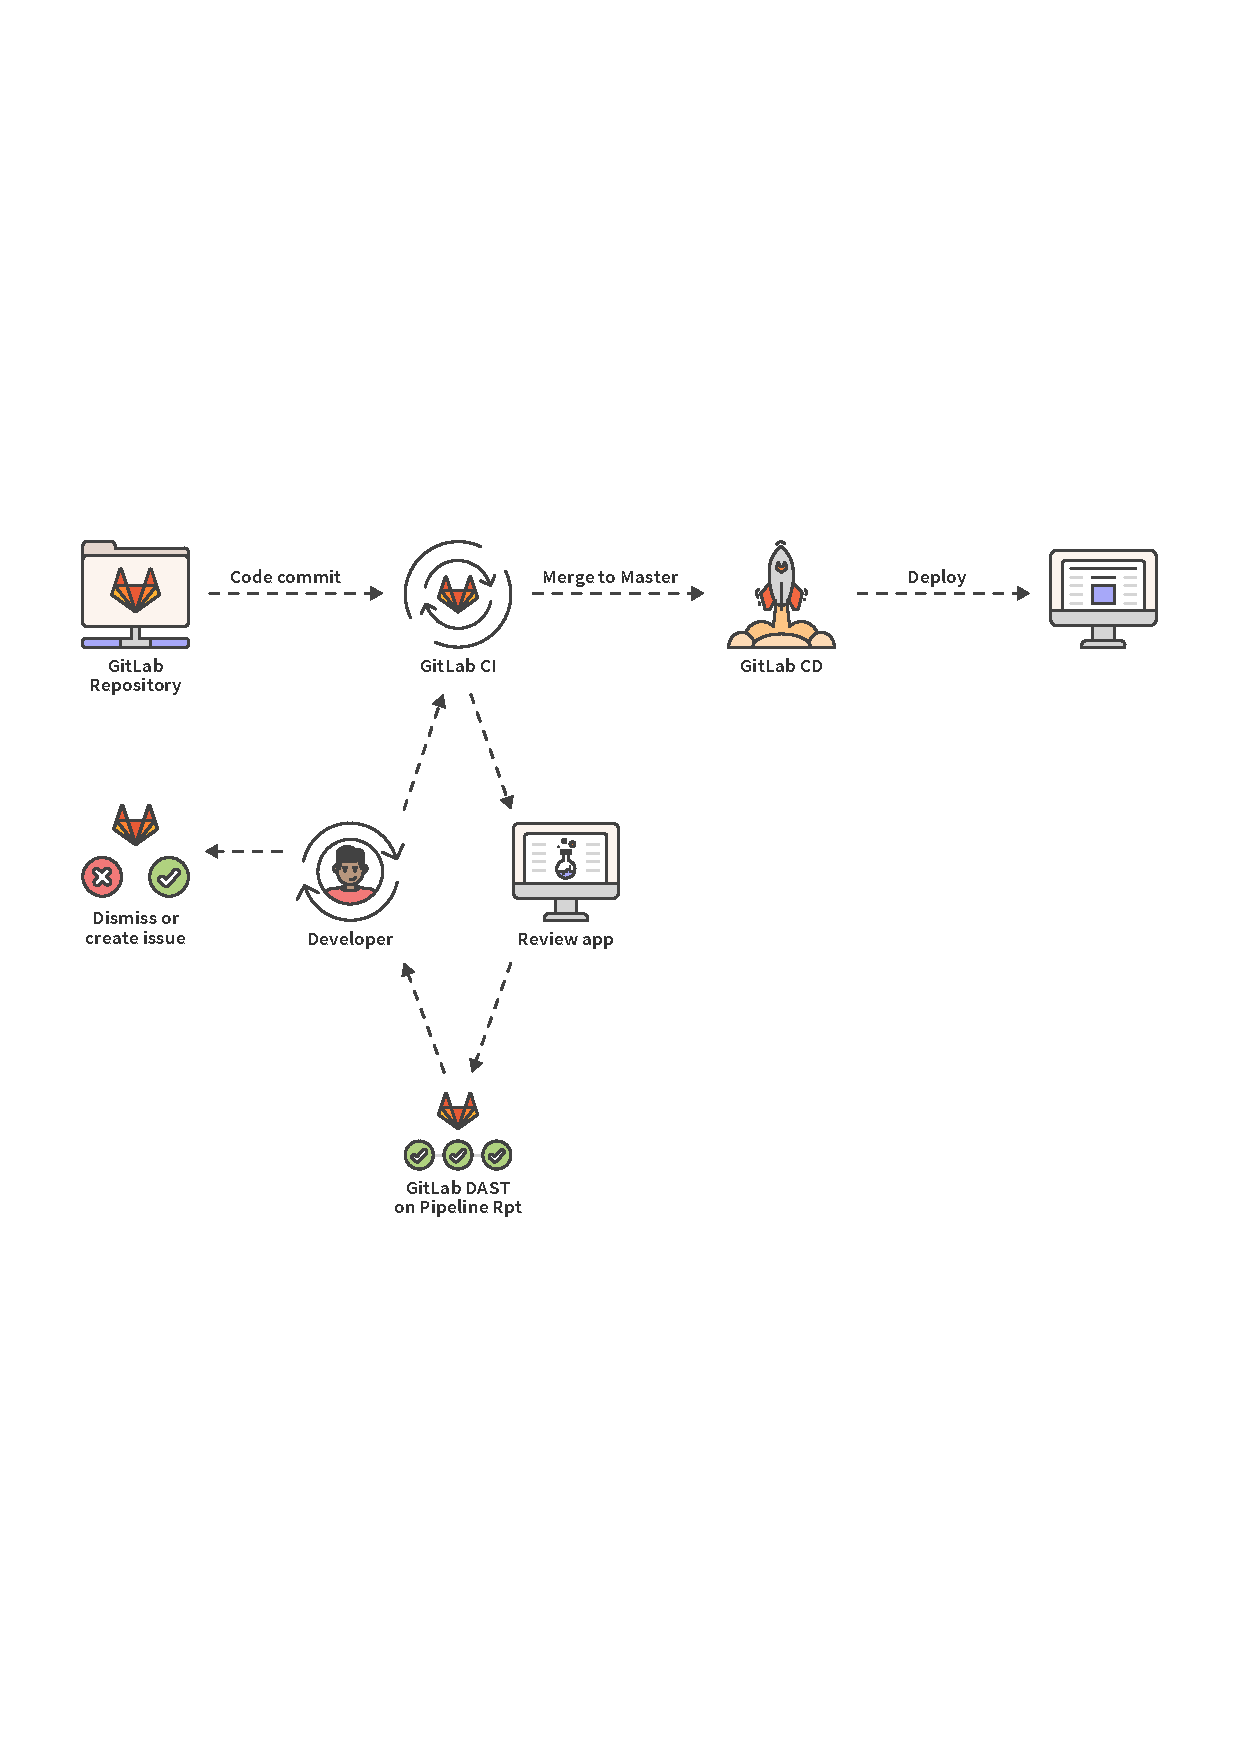
\includegraphics[width=\textwidth]{media/gitlab-review-cycle.pdf}
            \caption{Cyklus kontroly kvality aplikace GitLab s integrovaným \glstext{DAST} \cite{gitlab-app-security}. Vývojář může vyhodnotit bezpečnostní problémy před začleněním změň do sdíleného kódu.}
            \label{fig:gitlab-review-cycle}
        \end{figure}

        \todo{Jaké jsou historická CVE? Jaká je izolace klientů? Co aplikace potřebuje za přístupy?}\blind[1]

    \subsection{Dostupnost}
        S GitLabem mám praktické zkušenosti a provozuji ho pro přibližně 50 lidí. Zhruba 5 měsíců jsem používal balíček \textit{Omnibus} a s GitLab mikroslužbami pracuji podobně dlouho. Vyzkoušel jsem si i migraci z Omnibus na mikroslužby.

        Obě varianty nasazení byly při běžném používání (tzn. ne při správě) dobře dostupné. Většina výpadků nastala při problematických datech, které měly za následek extrémní zpomalení z pohledu uživatele. Jeden uživatel například nahrál $300$~MiB dump databáze a GitLab, resp. Gitaly, začal při počítání \textit{diff} padat. Jeden projekt tak omezil všechny ostatní projekty. GitLab by mohl mít nastavené lepší limity aby těmto výpadkům předešel, ideálně dynamicky podle dostupných zdrojů.

        \subsubsection{GitLab omnibus}
            Omnibus distribuce GitLabu, tedy balíček který obsahuje všechny komponenty, je primárně pro snadné nasazení a nepočítá se s tím, že by běžel s vysokou dostupností (\HA). Umožňují ale aktualizovat systém bez výpadku: doporučený postup je aktualizovat balíček, spustit databázové migrace a reloadnout webový frontend a konzumenty fronty \cite{gitlab-omnibus-update}. Důsledně se snaží dodržovat kompatibilitu napříč verzemi a databázové migrace dělají zpětně kompatibilní. V každém vydání nové verze jsou změny rozepsané a případné nekompatibility jsou znázorněny v tzv. \textit{upgrade barometer}.

            V základním nastavení nelze GitLab Omnibus replikovat. Některé komponenty lze ale vyčlenit. Nezbytné jsou PostgreSQL a Redis. Jediné co pak zbývá a sdílí se mezi replikami jsou samotné git repozitáře na souborovém úložišti. Vyzkoušel jsem, že GitLab Omnibus správně funguje ve víc replikách, když se vyčlení databáze a repozitáře se sdílí přes \glstext{NFS}. Jedná se ale o nezdokumentované nasazení a nemá oficiální podporu.

            Při nasazení ve víc replikách lze docílit 100 \% dostupnosti při aktualizaci na novější verzi.

        \subsection{GitLab microservices}
            \pfxref{Na diagramu}{pic:gitlab-architecture} (strana \pageref{pic:gitlab-architecture}) je znázorněna architektura GitLab mikroslužeb. Mikroslužby jsou obecně vhodné pro \glstext{HA} systémy:

            \begin{quote}
                [\ldots] each microservice in microservice architectures is operationally independent from others, and the only form of communication between services is through their published interfaces. This is fundamental since this allows one to change, fix or upgrade a microservice without compromising the system correctness, provided that the interfaces are preserved. \textit{Dragoni et al.~\cite{dragoni-microservices}}
            \end{quote}

            Klíčové komponenty GitLabu můžeme provozovat ve víc replikách a aktualizaci dělat pomocí rolling update, naprosto transparentně pro ostatní části systému. Některé komponenty jako jsou konzumenti fronty a manažer příchozích emailů můžeme dokonce aktualizovat s krátkým výpadkem, bez pozorovatelného dopadu pro uživatele.

            Správa stavových služeb je v distribuovaném systému nejkomplikovanější. GitLab jich bohužel používá celou řadu: relační databázi PostgreSQL, key-value storage Redis a vlastní služby Gitaly pro správu repozitářů. PostgreSQL s master-slave architekturou lze provozovat s vysokou dostupností použitím hot standby instance \cite{kim-postgres}. Redis také používá master-slave architekturu, ale dokáže si v případě výpadku sám zvolit v clusteru nový master díky komponentě Redis Sentinel \cite{redis-ha}. Tyto služby poskytovatelé cloudu nabízí i se správou, kde zodpovídají za dostupnost a některé aktualizace.

            Služba Gitaly je v oficiálním Helm chartu \glstext{SPOF}. Vystavuje \glstext{gRPC} \glstext{API} nad git repozitáři, se kterým pracuje většina ostatních komponent. Gitaly běží v jedné replice a je závislé na stavových datech na disku. Konzultoval jsem tento problém s oficiální podporou a je možné Gitaly provozovat nad \glstext{NFS} ve více replikách. Jde o kompromis mezi dostupností a rychlostí. Gitaly je z části limitováno propustností disku a \glstext{NFS} některé operace zpomalí.

            V oficiální distribuci má GitLab \glstext{SPOF} v Gitaly a při aktualizaci této komponenty je nedostupný. Při použití mikroslužeb s Gitaly nad \glstext{NFS} je GitLab bez výpadku dostupný pro použití i pro správu a dostupnost lze zvyšovat přidáním dalších replik.

    \subsection{Integrace}
        \todo{Integrace gitlabu, oznámení na GitHub/GitLab/Bitbucket/\ldots}\blind[2]
        \todo{Možnosti deploy z gitlabu do cílového systému; k8s, sftp, openstack, \ldots}\blind[5]

    \subsection{Praktické nasazení projektů}
        \subsubsection{Projekt 1}
            Nastavení pipeline pro statický projekt není vůbec přímočaré. Z webového rozhraní jsem vytvořil projekt včetně repozitáře, v lokálním git repozitáři jsem nastavil přidělený remote a zdrojové kódy jsem nahrál na GitLab. Potom jsem ručně napsal konfiguraci pipeline v souboru \code{.gitlab-ci.yml}. Protože jsem GitLab runner nasadil s executorem \code{shell}, nainstaloval jsem předem do sdíleného prostředí nezbytné závislosti. Popis instalace Ruby, Gem a balíčků Jekyll a Bundler jsem popsal \pfxref{v příloze}{ch:implementace}. Konfigurace GitLab pipeline obsahuje značné množství klíčových slov, ale má vynikající webovou dokumentaci. Uvítal jsem také podporu schématu v \glstext{IDE} IntelliJ IDEA \cite{idea-gitlab-plugin}, bez kterého se těžko s JSON pracuje.

            Pipeline jsem specifikoval dvoukrokovou. V prvním kroku se generují výstupy a výsledky se archivují jako tzv.~artefakty. V kroku druhém  se tyto artefakty stáhnou a nahrají na webový server. Díky tomuto rozdělení lze na GitLabu deploy opakovat bez nutnosti znovu generovat všechny artefakty. To umožňuje mj.~velmi rychlý rollback a obecně přesun mezi verzemi.

            Implementoval jsem podporu pro GitLab review apps. Změny z větve \code{deploy/prod} se automaticky nahrávají do produkčního prostředí. Ostatní větve se nasadí pro dynamicky vygenerovaného prostředí a vývojář je má po kontrole možnost ručně vypnout.

            Při použití \code{docker} executoru je pipeline stejně jednoduchá, ale odpadá nutnost předem nastavit prostředí a není nutné řešit kolize závislostí napříč projekty. GitLab dokáže artifacts ukládat z kontejneru stejně jako v \code{shell} executoru.

        \subsubsection{Projekt 2}
            Pipeline pro dynamický komplexní projekt je překvapivě podobná, jako u statického projektu. Opět jsem vytvořil dvě hlavní stage: build a deploy. Hlavní rozdíl je v samotných příkazech pro sestavení, které jsem abstrahoval do \code{Makefile}. Protože využívám \code{shell} executor, předinstaloval jsem \glstext{PHP}, balíčkovací systém composer a další. To je bohužel správa kterou je potřeba dělat mimo konfiguraci pipeline.

            Review apps jsem navrhnul teoreticky, protože bez kontejnerů je implementace zbytečně složitá. U relační databáze (ve smyslu \glstext{RDBMS}) je potřeba vytvořit novou databázi, nakonfigurovat oprávnění pro nového uživatele aby nemohl ovlivnit ostatní (a hlavně produkční) databáze, nakonfigurovat aplikaci aby používala jiné databázové údaje a spustit migrace. Dále je potřeba po ukončení review app nějakým způsobem tuto databázi smazat. Velmi podobný postup je potřeba opakovat pro key-value storage, na které je aplikace také závislá.

        \subsubsection{Projekt 3}
            Opět jsme použil úplně stejnou pipeline jako pro předchozí dva projekty. Pro sdílení vystavěného docker obrazu jsem použil GitLab Container Registry, což je vestavěná služba. Registr je automaticky založený při vytvoření GitLab projektu. V build scriptu jsem provedl authentikaci \code{docker login}. Heslo jsem hardcodoval rovnou do scriptu. Alternativně může být nastaveno ve webovém rozhraní GitLabu a předáno do jobu jako proměnná prostředí (\code{env}). To má smysl hlavně pro veřejné projekty, kde nechceme heslo zveřejňovat; pak je ale nutné ohlídat, aby \CI job nemohl kdokoliv škodlivě upravit, spustit, a nechat si vypsat heslo do logu.

            Pro build aplikace se používá hostitelský docker démon. Celou řadu výhod a nevýhod a alternativní řešení jsem rozepsal \pfxref{v sekci o Dockeru}{sec:gitlab-ci-docker}.

            Pro spuštění aplikace na webovém serveru se nejprve nahraje soubor pro konfiguraci Docker Swarm stacku. Na webovém serveru se pak spustí přihlášení do registru a příkazem \code{docker stack deploy} se spustí a případně aktualizuje aplikace.

            U tohoto ukázkového projektu si použitím \code{docker} executoru moc nepomůžeme. Docker jako závislost musí být na hostitelském serveru předinstalovaný a pro zbytek se používají kontejnery.
